\documentclass{article}
\usepackage{graphicx} % Required for inserting images
\usepackage[title]{appendix}
\usepackage{amsmath}
\usepackage{circuitikz}
\usepackage{hyperref}
\usepackage{caption}
\begin{titlepage}
   \begin{center}
       \vspace*{1cm}
       \huge
       \textbf{Time and frequency domain analysis of a low-pass $RC$-filter}\\
       \vspace{1.5cm}
        \large
       Gabriel Mazili Pedroza -- gmp40, lab group 47\\
       \vspace{0.5cm}
       11 November 2024\\
       \vspace{0.5 cm}
       \textit{Homerton College, University of Cambridge}
       \vspace{1.5 cm}
        \begin{abstract}
            As part of the coursework for the Integrated Electrical Project, the features of a low-pass $RC$-filter were dimensioned with an oscilloscope. The aims were to compare the measured characteristic time $\tau$ and attenuation curve (including its roll-off) to the theoretical predictions, to quantify the impact of component tolerances in gathered data, and to test if $\tau$ values chosen within said tolerances could improve the agreement with theory. The attenuation data matched theory without theoretical adjustments, but changes to the idealised circuit model were required to enhance agreement in the transient response experiment. Furthermore, choosing an \textit{ad hoc} value for $\tau$ improved the agreement in both cases, although its closeness to the nominal value meant the impact of tolerances on circuit behaviour were largely unobserved in experiments. 
        \end{abstract}
       \vfill
            
   \end{center}
\end{titlepage}
\begin{document}
\captionsetup{font=small}
\newcommand{\Vout}{V_{\text{out}}}
\newcommand{\Vin}{V_{\text{in}}}
\newcommand{\Vusb}{V_{\text{USB}}}
\newcommand{\vout}{v_{\text{out}}}
\newcommand{\Vmax}{V_{\text{max}}}
\newcommand{\vin}{v_{\text{in}}}
\newcommand{\vinr}{v_{\text{in}}^{\text{RMS}}}
\newcommand{\voutr}{v_{\text{out}}^{\text{RMS}}}
\newcommand{\td}{t_\text{d}}

\section{Introduction and Objectives}
As part of the Physical Principles of Electronics class, the electrical features of a theoretical capacitor were discussed in detail. This allowed for the prediction both of its transient behaviour while charging under a resistor, and of the attenuation offered to AC signals when part of a low pass $RC$-filter.
\par However, electrolytic capacitors are different from their theoretical counterparts, as they are polarised and have imperfect insulation between its conductors. Furthermore, both resistors and capacitors are subject to manufacturing tolerances which can impact the agreement between calculated and measured behaviour. None of this was directly explored in the theoretical lectures, thus justifying these experiments.
\par Therefore, the goal of the experiments was to quantify the difference between the expected and the measured values for the characteristic time and attenuation profiles of a $RC$-filter. Moreover, the experiments also aim at measuring the impact of component tolerances in circuit behaviour. In particular, it is to be tested how much choosing a non-nominal value for $\tau$ within said tolerances improves agreement between data and theory.
\section{Experimental Method}
For both experiments, it was used a carbon film resistor of resistance $R = 100 \text{ k}\Omega \pm 5\%$ and an electrolytic capacitor of capacitance $C = 1 \text{ }\mu\text{F} \pm 20\%$. Further details can be found in the respective handouts for Exercise B and C.
\subsection{Transient response}
The circuit was arranged as shown in Figure \ref{fig:transient}. The \textit{LED} was used as a power indicator in accordance with the guide in Exercise B, and its effects in the measurements are negligible. The power was implemented by a standard \textit{USB} supply, whose voltage was measured at $\Vusb = 5.15 \text{ V}$. The switch was a wire which was plugged into the correct breadboard hole in order to close the circuit. Finally the capacitor was manually discharged by shorting its legs between measurements, in order to avoid unintended influences between runs.
\begin{figure}[!htb]
\centering
    \begin{circuitikz}
        \tikzstyle{every node}=[font=\large]
        \draw (5,10.5) to[short] (6.5,10.5);
        \draw (6.5,8.5) to[empty led] (6.5,7);
        \draw (6.5,10.5) to[european resistor,l={ \large 100 k$\Omega$}] (9.5,10.5);
        \draw (9.5,10.5) to[normal open switch] (9.5,8.25);
        \draw (9.5,8.5) to[short, -o] (11.5,8.5) ;
        \draw (6.5,7) to[short] (6.5,6.5);
        \draw (5,6.5) to[short] (6.5,6.5);
        \draw (9.5,8.25) to[curved capacitor,l={ \large 1 $\mu$F}] (9.5,6.5);
        \draw (6.5,6.5) to[short] (9.5,6.5);
        \node at (6.5,10.5) [circ] {};
        \node at (6.5,6.5) [circ] {};
        \draw (6.5,10.5) to[european resistor,l={ \large 10 k$\Omega$}] (6.5,8.5);
        \draw (9.5,6.5) to[short, -o] (11.5,6.5) ;
        \draw [->, >=Stealth] (11.5,7) -- (11.5,8)node[pos=0.5,right, fill=white]{$\Vout$};
        \draw (5,10.5) to[short] (4.25,10.5);
        \draw (5,6.5) to[short] (4.25,6.5);
        \draw (4.25,10.5) to[american voltage source,l={ \large 5 V}] (4.25,6.5);
    \end{circuitikz}
    
    \caption{Circuit diagram with nominal values used to measured the transient response of the filter.}
    \label{fig:transient}
\end{figure}
\par Every run, the capacitor would start discharged and with the switch open. Then, the switch would be closed, and the voltage of the capacitor would be measured by a one-shot oscilloscope through a $1\text{ M}\Omega$ probe, capturing its charging curve.
\subsection{AC attenuation}
For the AC attenuation measurements, the circuit was arranged as shown in Figure \ref{fig:ac}. For the supply, it was used the wave generator of the oscilloscope itself, set to an amplitude of $1 \text{ V}$, and a DC offset of $1$ V too, in order to meet the polarity of the capacitor. The probes were set to $10\times1\text{ M} \Omega = 10 \text{ M}\Omega$ of impedance, and the oscilloscope was set to ``AC Mode" so as to neglect DC offsets in the measurements.
\begin{figure}[!htb]
\centering
    \begin{circuitikz}
        \tikzstyle{every node}=[font=\large]
        
        \draw (4.25,10.5) to[european resistor,l={ \large 100 k$\Omega$}] (9.5,10.5);
        %draw (9.5,10.5) to[short] (9.5,8.25);
        \draw (9.5,10.5) to[short, -o] (11.5,10.5) ;
        
        \draw (4.25,6.5) to[short] (6.5,6.5);
        \draw (9.5,10.5) to[curved capacitor,l={ \large 1 $\mu$F}] (9.5,6.5);
        \draw (6.5,6.5) to[short] (9.5,6.5);
        
        
        \draw (9.5,6.5) to[short, -o] (11.5,6.5) ;
        \draw [->, >=Stealth] (11.5,7) -- (11.5,10)node[pos=0.5,right, fill=white]{$\vout$};
        \draw (4.25, 10.5) to[short, -o] (2.25, 10.5);
        \draw (4.25, 6.5) to[short, -o] (2.25, 6.5);
        \draw [->, >=Stealth] (2.25,7) -- (2.25,10)node[pos=0.5,left, fill=white]{$\vin$};
        
        \draw (4.25,10.5) to[vsourcesin,l={ \large 1 V}] (4.25,6.5);
    \end{circuitikz}
    
    \caption{Circuit diagram with nominal values used to measured the AC response of the filter.}
    \label{fig:ac}
\end{figure}
\par Since AC response was being measured, there was no need to discharge the capacitor between runs. For each frequency, the oscilloscope (in one-shot mode) directly measured the AC root-mean-square (RMS) ripple voltage of both $\vin$ and $\vout$ in order to compute the attenuation.
\section{Theory}
\subsection{Transient response}
For a capacitor $C$ charging under a constant power supply $\Vusb$ with a resistor $R$ in series, Kirchhoff's Voltage Law dictates that
\begin{equation*}
    \begin{split}
        \Vusb &= RI + \frac{Q}{C} = RI + \Vout,
    \end{split}
\end{equation*}
where $Q$ denotes the capacitor's charge at any point in time and $I$ the current through the circuit. The solution of the above equation is straightforward, and substituting for the boundary condition of the experiment, namely $\Vout(0) = 0$, gives:
\begin{equation}
    \Vout(t) = \Vusb\left( 1 - e^{-t/RC}\right).
    \label{eqn:charge_ideal}
\end{equation}
Naturally, $\tau = RC$ is defined as the characteristic time of the system, such that $\Vout(\tau) \approx 0.63 \cdot\Vusb.$
\par Due to manufacturing tolerances, the value of $\tau$ can be expected to vary between $(1-5\%)\cdot(1-20\%) = 76\%$ and $(1+5\%)\cdot(1+20\%) = 126\%$ of its nominal value. Therefore, substituting the values for the components, it is obtained that
\begin{equation}
    76\text{ ms} \le \tau \le 126 \text { ms}
    \label{eqn:tau_boundary}
\end{equation}
for the experiment.
\subsection{AC attenuation}
Let an oscilloscope supply a voltage given by $\Vin(t) = A\cos(\omega t) + B$ to a resistor $R$ in series with a capacitor $C$. As the equations governing the circuit are linear, the DC offset $B$ can be separated from the AC signal $\vin(t) = A\cos(\omega t)$; in particular, as the oscilloscope was set to measure only AC signals, $B$ can be safely ignored. Furthermore, the steady state of the system shall be analysed, allowing for the use of impedances to compute the expected behaviour of the capacitor.
\par For the purposes of the experiment, the circuit can be thought of as a voltage divider. The voltage in the capacitor then becomes
\begin{equation*}
    \vout^*= \vin^*\frac{1/j\omega C}{R + 1/j\omega C},
\end{equation*}
where starred variables denote complex counterparts to the real variables (i.e. $\vin^* = A\exp(j\omega t)$, etc.) Then the RMS value can be computed in a straightforward manner, viz.
\begin{equation*}
        \vout^{\text{RMS}} = \left[\frac{1}{2\pi}\int\limits_0^{2\pi}\left|\vin^*\frac{1/j\omega C}{R + 1/j\omega C}\right|^2dt\right]^{1/2} = \frac{1}{\sqrt{1 + (\omega RC)^2}} \vinr.
\end{equation*}
The attenuation in decibels is then given by
\begin{equation}
    20\log\left(\frac{\voutr}{\vinr}\right) = -10\log\left(1 + (\omega RC)^2\right),
    \label{eqn:ac_plot}
\end{equation}
yielding a roll-off estimated at
\begin{equation}
\begin{split}
        -10\log\left(1 + (10\cdot\omega RC)^2\right) - \left[-10\log\left(1 + (\omega RC)^2\right)\right] &= 10\log \left(\frac{1 + (\omega RC)^2}{1 + (10\cdot\omega RC)^2} \right)\\
        \\
        &\sim-20 \text{ dB/decade}
\end{split}
\label{eqn:roll_off}
\end{equation}
in the asymptotic limit of large frequencies. Remarkably, the roll-off is independent of the precise values of the resistor and of the capacitor. Therefore, it is expected that its measured value stays within the imprecision of the oscilloscope, which is small. 
\section{Results}
\subsection{Transient response}
The measurement of the transient response as outlined in the Experimental Method section returned the data as presented in Figure \ref{fig:transient_graph} (a complete table of experimental data is given in the appendix). A plot of the theoretical model derived during the Theory section is present in red for comparison purposes.
\begin{figure}[!htb]
    \centering
    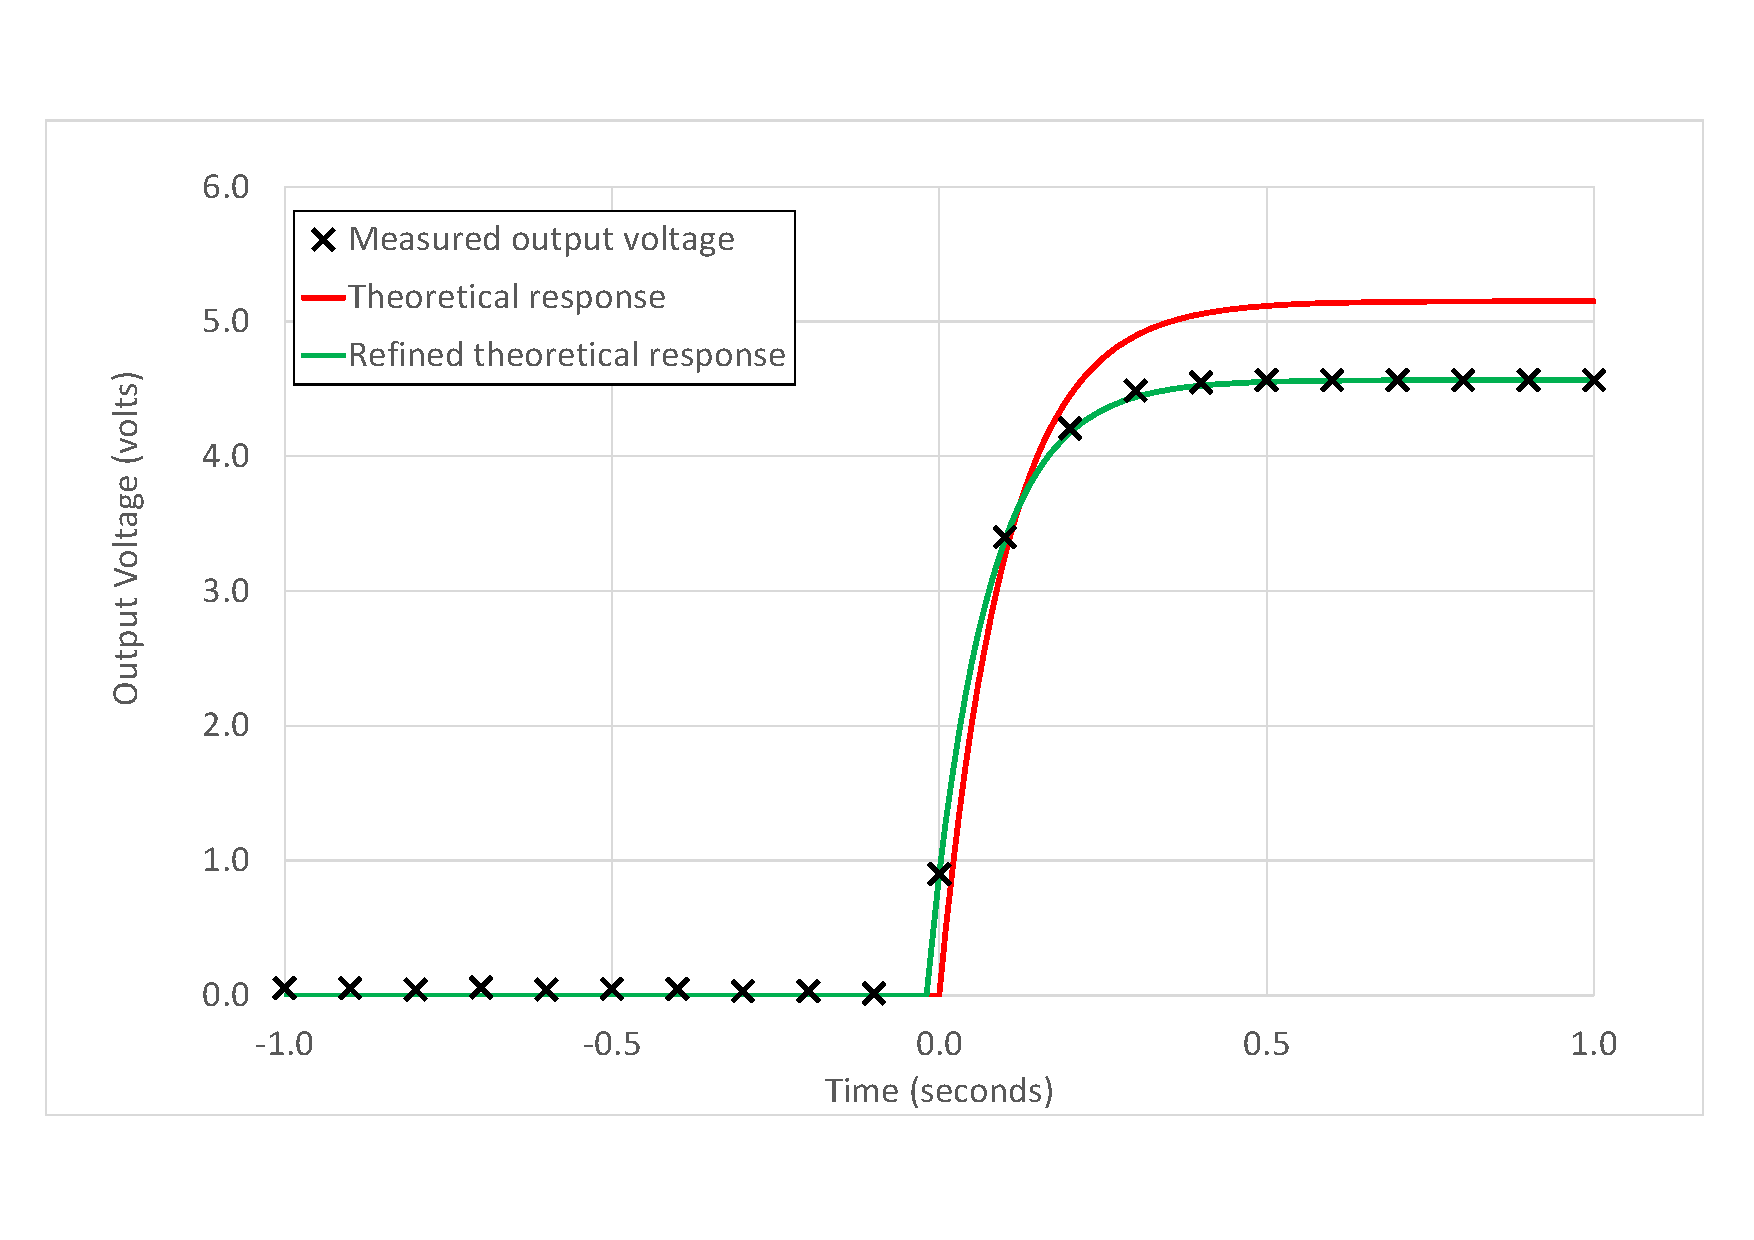
\includegraphics[width = \linewidth]{transient_graph.pdf}
    \caption{Graph comparing the measured $\Vout$ with two predicted models: one given by the discussion in the Theory section, and one adjusted to account for non-idealities in the experimental setup.}
    \label{fig:transient_graph}
\end{figure}
It must be noted that the oscilloscope trigger was set to 1 V, so that the experimental $t = 0\text{ s}$ is slightly different from the theoretical assumption. To account for this, a time offset $\td$ is to be added to a refined theoretical model $\Vout(t) \to \Vout(t - \td)$. In order to calculate $\td$, the fact that $\Vout(0)$ is known is used:
\begin{equation}
    \Vout(0) = \Vusb \left[1 - \exp\left(-\frac{0-\td}{\tau}\right)\right] \iff \td = \tau\ln\left(1-\frac{\Vout(0)}{\Vusb}\right).
    \label{eqn:td}
\end{equation}
Furthermore, a simple analysis of the data suggests that the maximum attainable voltage $\Vmax$ is not the $\Vusb$ predicted from theory. This cannot be explained without changes to the model circuit, as the maximum voltage is not influenced by $\tau$. Indeed, this happens because the combined finite resistances of the probe and of the capacitor create an effective resistor across the capacitor, as shown in Figure \ref{fig:transient_corrected}. 
\begin{figure}[!htb]
\centering
    \begin{circuitikz}
        \tikzstyle{every node}=[font=\large]
        \draw (5,10.5) to[short] (6.5,10.5);
        \draw (6.5,8.5) to[empty led] (6.5,7);
        \draw (6.5,10.5) to[european resistor,l={ \large 100 k$\Omega$}] (9.5,10.5);
        \draw (9.5,10.5) to[normal open switch] (9.5,8.25);
        \draw (9.5,8.5) to[short] (11.5,8.5) ; %a
        \draw (6.5,7) to[short] (6.5,6.5);
        \draw (5,6.5) to[short] (6.5,6.5);
        \draw (9.5,8.25) to[curved capacitor,l={ \large 1 $\mu$F}] (9.5,6.5);
        \draw (6.5,6.5) to[short] (9.5,6.5);
        \node at (6.5,10.5) [circ] {};
        \node at (6.5,6.5) [circ] {};
        \draw (6.5,10.5) to[european resistor,l={ \large 10 k$\Omega$}] (6.5,8.5);
        \draw (9.5,6.5) to[short] (11.5,6.5) ;%b
        \draw (11.5, 8.5) to[european resistor, l = {\large 780 k$\Omega$}] (11.5, 6.5);
        \draw (11.5, 8.5) to[short, -o] (13.5, 8.5) ;
        \draw (11.5, 6.5) to[short, -o] (13.5, 6.5) ;
        \draw [->, >=Stealth] (13.5,7) -- (13.5,8)node[pos=0.5,right, fill=white]{$\Vout$};
        \draw (5,10.5) to[short] (4.25,10.5);
        \draw (5,6.5) to[short] (4.25,6.5);
        \draw (4.25,10.5) to[american voltage source,l={ \large 5 V}] (4.25,6.5);
    \end{circuitikz}
    
    \caption{Corrected transient circuit to account for finite impedance across capacitor.}
    \label{fig:transient_corrected}
\end{figure}
\par From the data, the value of the effective resistor can be calculated through a simple potential divider equation at
\begin{equation}
    R_\text{eff} = 100\text{ k}\Omega\cdot\frac{\Vmax}{\Vout - \Vmax} \approx 780\text{ k}\Omega,
    \label{eqn:reff}
\end{equation}
since in the steady state the current through the capacitor can be treated as null. However, the modified circuit also has different circuit dynamics, viz.
\begin{equation*}
    \begin{split}
        \frac{Q}{C} &= R_\text{eff}(I -i)\\
        \Vusb &= 100\text{ k}\Omega\cdot I + R_\text{eff} (I - i),
    \end{split}
\end{equation*}
where $I$ denotes the current from the supply and $i$ the current through the capacitor. The solution is also straightforward, and it can be seen that
\begin{equation}
    \tau_\text{eff} = \frac{100 \text{ k}\Omega \cdot R_\text{eff}}{100 \text{ k}\Omega + R_\text{eff}} C \approx 89\text{ ms}.
    \label{eqn:correct_tau}
\end{equation}
Substituting (\ref{eqn:td}) and (\ref{eqn:correct_tau}) into a complete equation, the corrected theoretical prediction is
\begin{equation*}
    \Vmax(t) = \Vmax \left[1 - \exp \left(-\frac{t-\td}{\tau_\text{eff}}\right) \right],
\end{equation*}
which is plotted with a green line in Figure \ref{fig:transient_graph}. Whereas the RMS error of the initial theoretical fit is around $398$ mV, the RMS error of the new fit is around $34.1$ mV.
\subsection{AC attenuation}
The data collected by the experiment detailed in the Experimental Method section can be found in Figure \ref{fig:ac_graph}, along with a fit based on the Theory section. The RMS error of the fit measures at around $0.380 \text{ dB}$. A complete table of the data is presented in the appendix. 
\begin{figure}
    \centering
    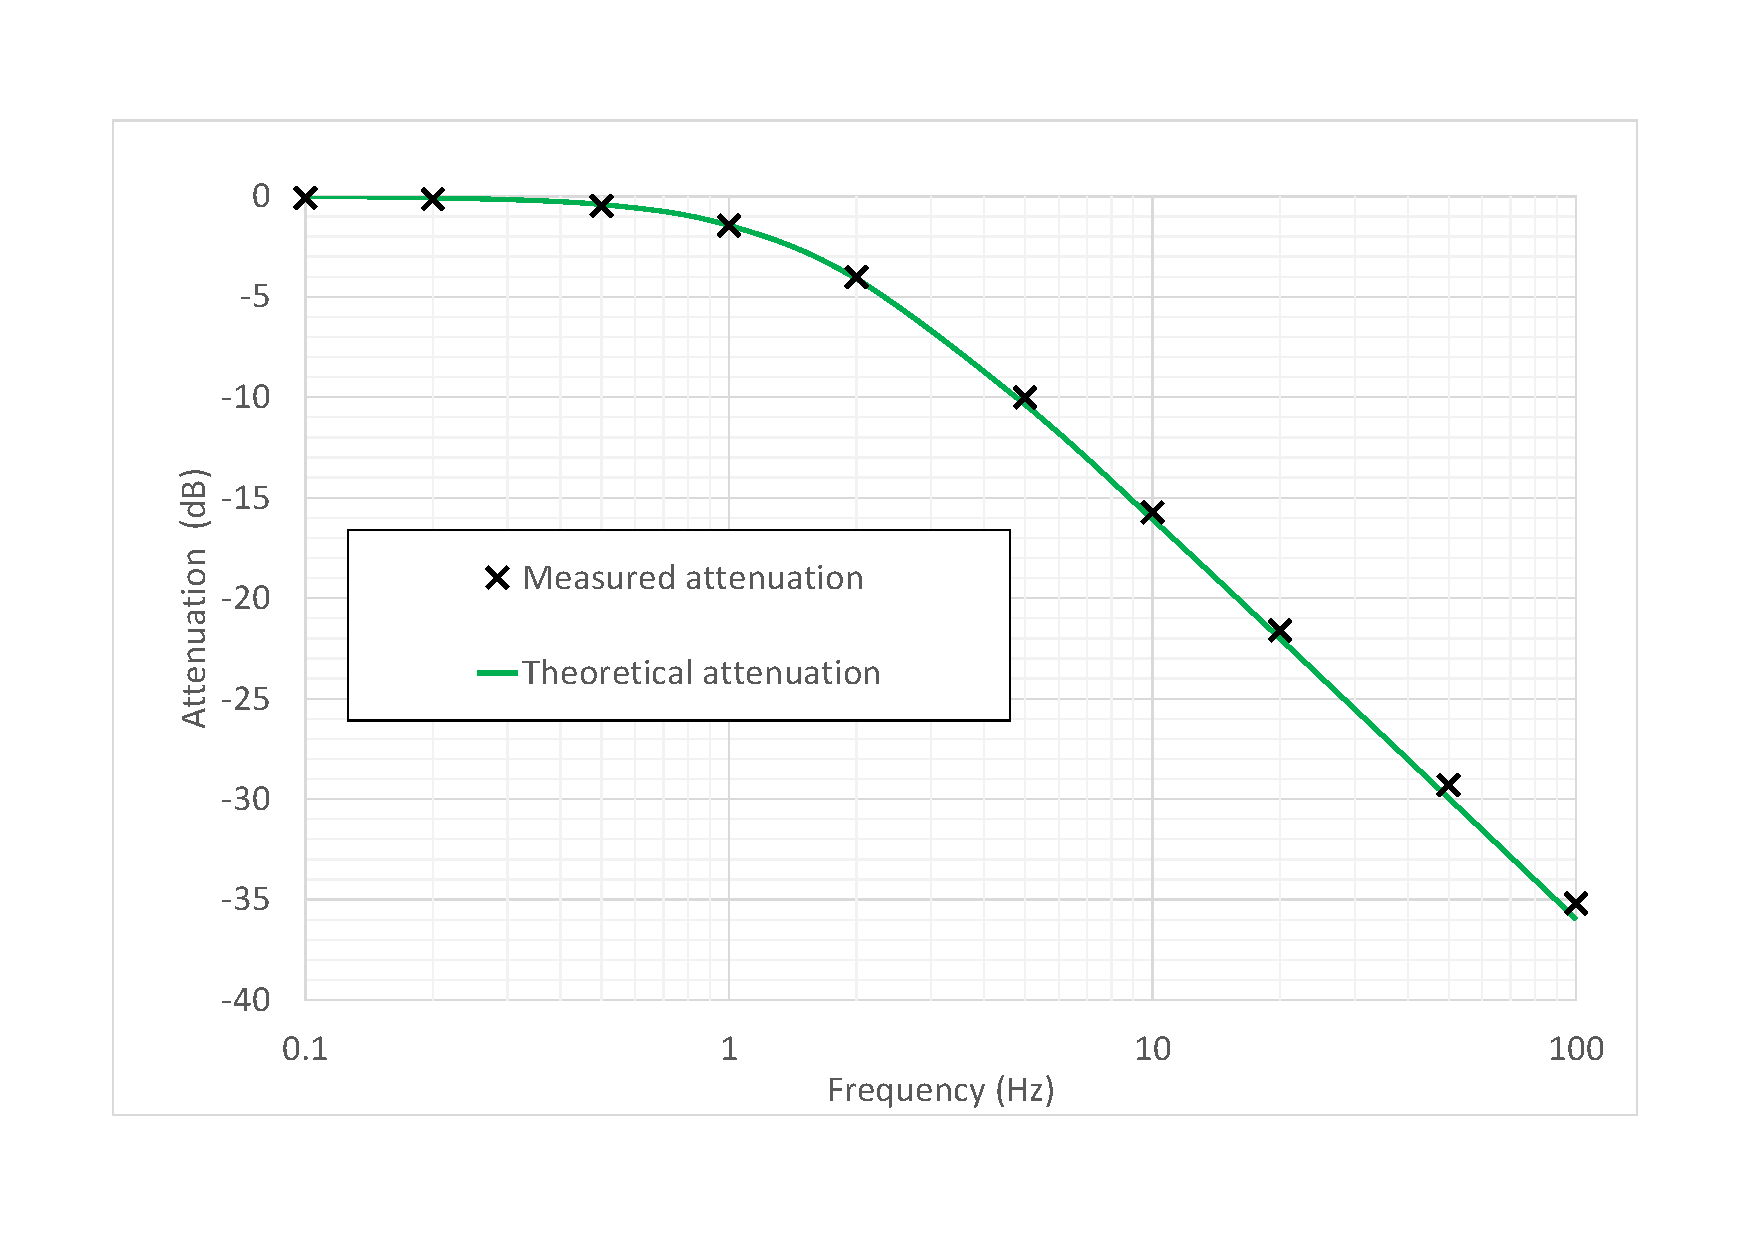
\includegraphics[width=\linewidth]{ac_graph.pdf}
    \caption{Attenuation of the low-pass $RC$-filter as a function of frequency, plotted against a plain theoretical model.}
    \label{fig:ac_graph}
\end{figure}
\par Because the attenuation was measured with a $10 \text{ M}\Omega$ probe, and the leakage current of the capacitor is negligible (as hinted by the result of (\ref{eqn:reff}), which is close to the rated impedance of the oscilloscope), it is expected that the previously presented model for this circuit suffices to explain the results. Therefore, a refined theoretical model is not drafted. 
\section{Discussion}
Both the AC attenuation and the transient response experiments showed close agreement with the theoretical model, without any significant deviations. 
\par The reader can readily see that the theoretical attenuation, in particular the roll-off predicted in (\ref{eqn:roll_off}), is observed with great accuracy in the experimental data of Figure \ref{fig:ac_graph}. This agreement is quantified by the small RMS error of $0.380 \text{ dB}$ across the fit. This can be improved in an \textit{ad hoc} manner by choosing a $\tau$ value still in the boundaries imposed by (\ref{eqn:tau_boundary}) that minimises the RMS error. Indeed, it seems that a value of $\tau ' \approx 95\text{ ms}$ gives a closer fit, with RMS error of  $0.151 \text{ dB}$, whose slightly different plot can be seen in Figure \ref{fig:ac_graph_corrected}.
\begin{figure}[!htb]
    \centering
    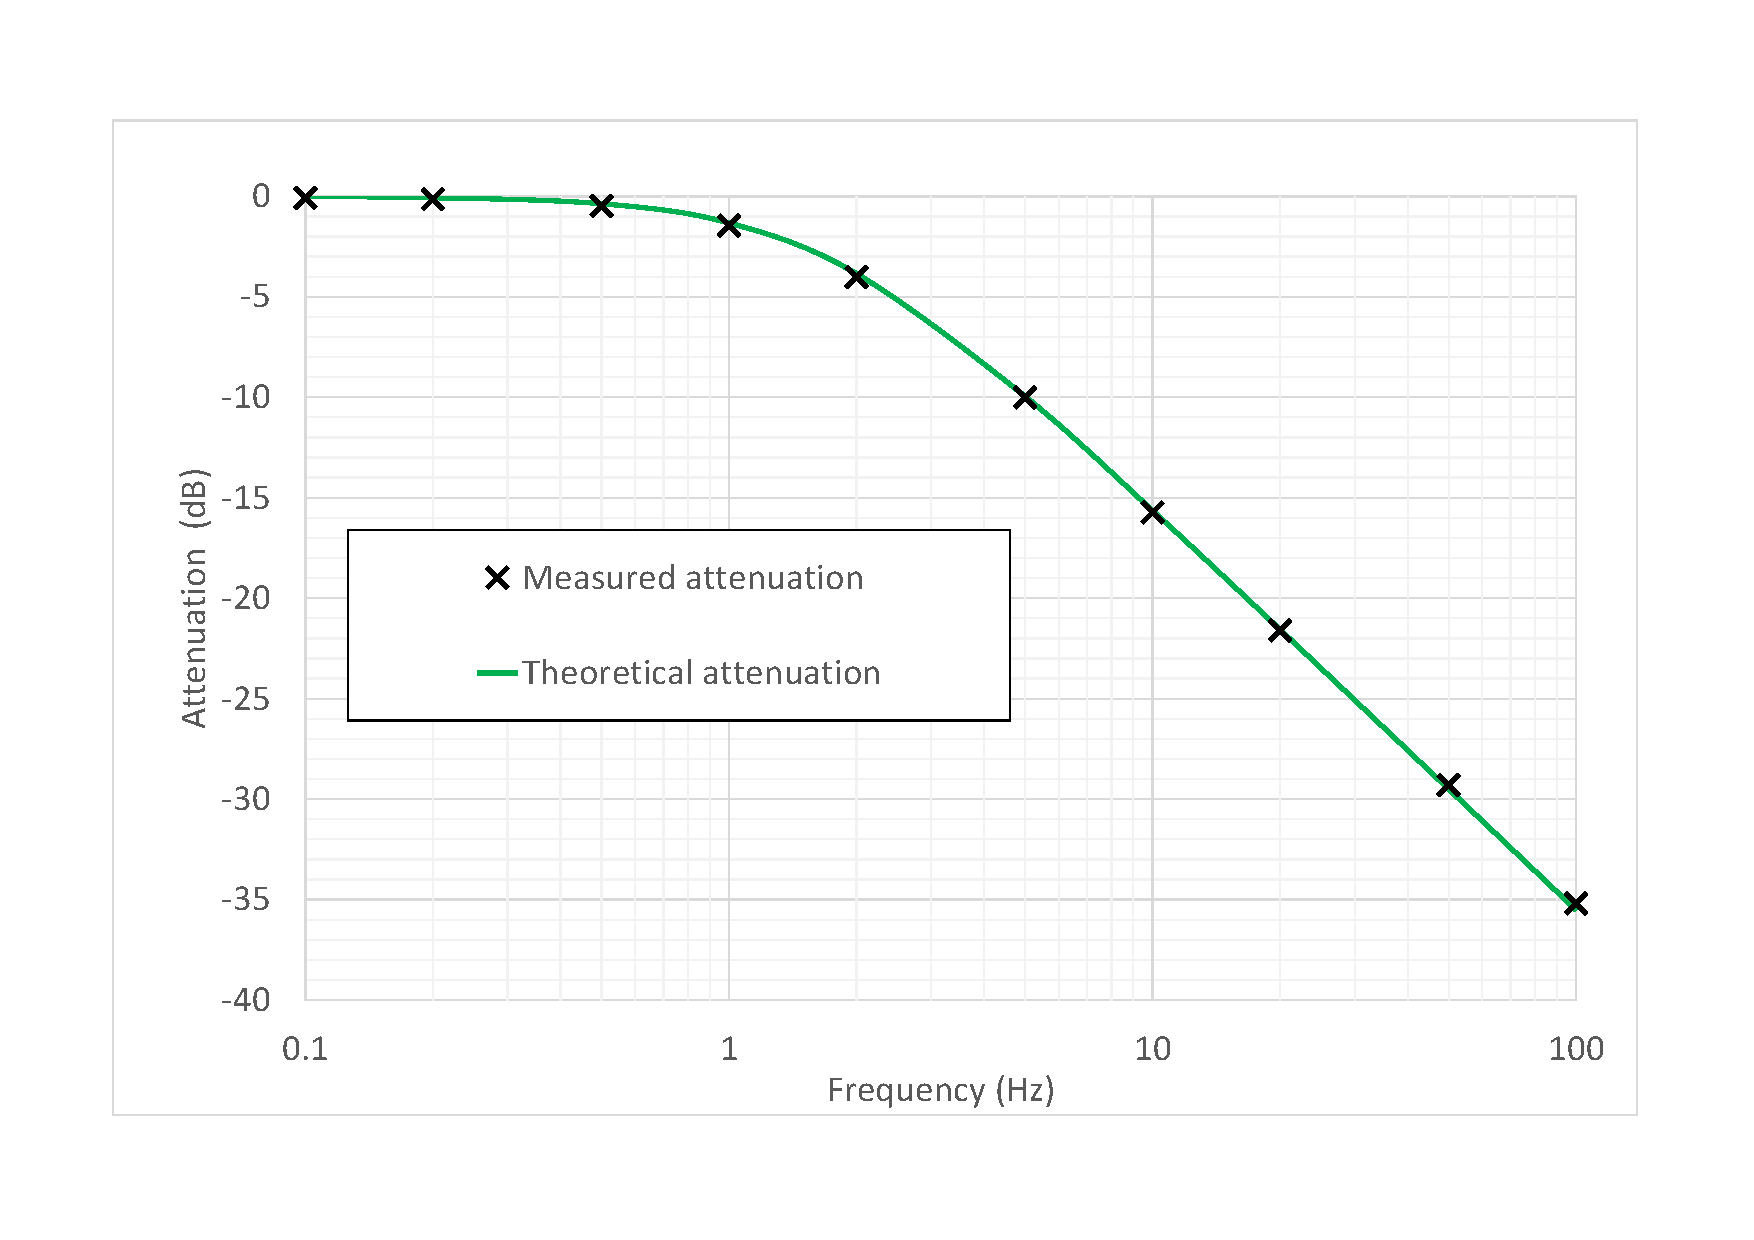
\includegraphics[width=\linewidth]{ac_graph_corrected.pdf}
    \caption{AC attenuation graph with the improved value of $\tau' = 95\text{ ms}$ for the theoretical fit. Notice how the agreement between theory and data is closer vs. Figure \ref{fig:ac_graph}, especially in the higher frequency range.}
    \label{fig:ac_graph_corrected}
\end{figure}
\par The transient response measured deviated significantly from the original expected theoretical model, and trivial time-alignment corrections would be insufficient to account for the unanticipated RMS error of $398$ mV. A much more comprehensive overhaul of the theory was needed to reduce the RMS error to $34.1$ mV, taking into account the finite impedance of the oscilloscope. This correction, although sufficient to explain the experimental results, can be further refined through the adoption of $\tau'$ found above into the theoretical model. This yields a slightly smaller RMS error of $33.7$ mV, producing a different fit that is nevertheless too similar to the original one to justify its inclusion in this report.  
\section{Conclusions}
\begin{enumerate}
    \item The measured performance (both transient and AC) of the low-pass $RC$-filter matched closely that expected due to theory, although some theoretical corrections were needed to account for the physical experimental setup in the transient experiment;
    \item The expected -20 dB/decade filter roll-off approximated the measured value with great accuracy
    \item The tolerances of the capacitor and of the resistor were found to impact the attenuation values more than the transient response, although in the particular experimental setup used the actual value for $\tau$ was very close to nominal. It thus remains inconclusive whether larger differences could yield widely different results.
    \item It was found that choosing an \textit{ad hoc} value for $\tau$ within the tolerances managed to improve the agreement between theory and data, particularly in the AC attenuation prediction.
\end{enumerate}
\begin{appendices}
\section{Complete dataset}
    \begin{itemize}
        \item Data for transient response: \\\url{https://drive.google.com/file/d/1xkVoVKPQf44SvPc_8-n4ES4F0VvzIOdi/view?usp=sharing}
        \item Data for AC attenuation: \\
        \url{https://docs.google.com/spreadsheets/d/1DedUJOme2nNKu-LPahmzVtML57rTUMDswer1W_CGQ3w/edit?usp=sharing}
    \end{itemize}
\end{appendices}
\end{document}
